% withpage: ページ番号をつける (著者確認用)
% english: 英語原稿用フォーマット
\documentclass{ipsjprosym}
%\documentclass[withpage,english]{ipsjprosym}

\usepackage[dvipdfmx]{graphicx}
\usepackage{latexsym}

\begin{document}

% Title, Author %%%%%%%%%%%%%%%%%%%%%%%%%%%%%%%%%
\title{環境にメソッドを直接格納する \\ 新しいオブジェクトシステムの提案}

\affiliate{COINS}{筑波大学情報学群情報科学類}
\affiliate{CS}{筑波大学システム情報系}

\author{林 拓人}{Takuto Hayashi}{COINS}[hayashi@ialab.cs.tsukuba.ac.jp]
\author{前田 敦司}{Atusi Maeda}{CS}[maeda@cs.tsukuba.ac.jp]

\begin{abstract}
[概要(400字程度)]TODO:構成を決めた後全体を要約する
\end{abstract}

\begin{jkeyword}
オブジェクトシステム,メソッド,クラス,総称関数,環境
\end{jkeyword}

\maketitle

% Body %%%%%%%%%%%%%%%%%%%%%%%%%%%%%%%%%
\section{序論}

従来のクラスベース・オブジェクトシステムをメソッドの格納方式に着目してモデル化すると,
次の2つのモデルに分類することができる.
1つはクラスにメソッドを格納するモデル,もう1つはCLOS\cite{CLOS}のように総称関数にメソッドを
格納するモデルである.

本論文は,これら2つの格納モデルに対する分析に基づき考案した,全く新しい格納モデルを持つ
オブジェクトシステムを提案する.
また,その特徴を最大限に生かせるよう独自に設計したプログラミング言語Suzuを用いて,提案する
オブジェクトシステムの評価を行う.

\section{従来のオブジェクトシステム}

ここではモデルを単純化するため,多重ディスパッチについては考えないものとする
(TODO:多重ディスパッチについて述べている節へのrefを挿入).

\subsection{クラスにメソッドを格納するモデル}

クラスにメソッドを格納するモデルでは環境にクラスを格納し,クラスにメソッドを格納する
(図\ref{fig:classes}).
ここで環境はクラス名をキーとしてクラスを格納する辞書であり,クラスはメソッド名をキーとして
メソッドを格納する辞書である.
SmalltalkやRubyなどのオブジェクトシステムはこのモデルに分類される.


\subsection{総称関数にメソッドを格納するモデル}

総称関数にメソッドを格納するモデルでは環境に総称関数を格納し,総称関数にメソッドを格納する
(図\ref{fig:generic-functions}).
ここで環境はメソッド名をキーとして総称関数を格納する辞書であり,総称関数はクラス名をキーとして
メソッドを格納する辞書である.
CLOSはこのモデルに分類される.

\begin{figure}
\centering
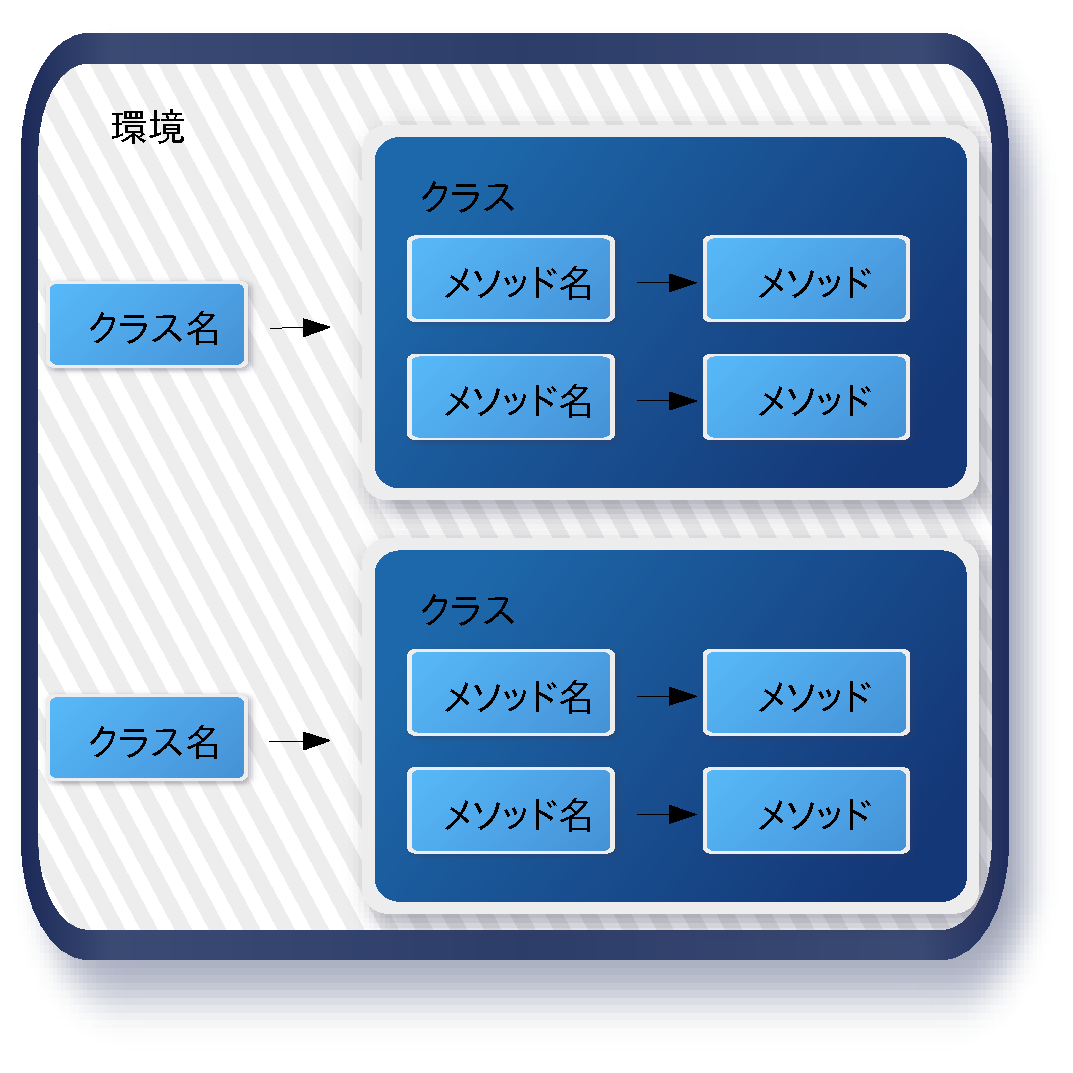
\includegraphics[width=7cm]{fig/classes-crop.pdf}
\caption{クラスにメソッドを格納するモデル}
\label{fig:classes}
\end{figure}

\begin{figure}
\centering
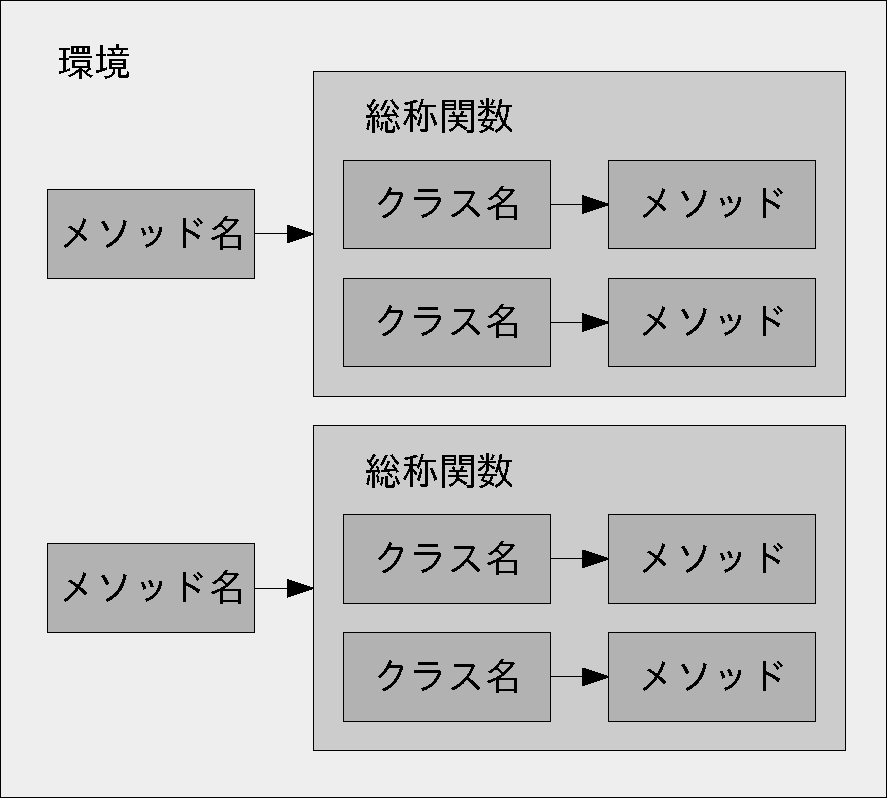
\includegraphics[width=7cm]{fig/generic-functions-crop.pdf}
\caption{総称関数にメソッドを格納するモデル}
\label{fig:generic-functions}
\end{figure}

\section{提案するオブジェクトシステム}

従来のオブジェクトシステムの分類先である2つのモデルは,どちらもクラス名とメソッド名が決まれば
メソッドが一意に定まるという特徴を持つ.
また,環境という辞書の中にクラスあるいは総称関数という辞書が入れ子になっている構造も
共通している.

提案するオブジェクトシステムはこのようなクラスや総称関数による入れ子構造を廃し,
\textbf{環境にメソッドを直接格納する}モデルを採用する(TODO:図の挿入).
ここで環境は\textbf{クラス名とメソッド名の組}をキーとしてメソッドを格納する辞書である.

このモデルの特徴は,メソッドの格納方式が一般的な変数の格納方式と類似していることである.
メソッドがクラス名とメソッド名の組をキーとして環境に格納されるのに対し,変数は変数名を
キーとして環境に格納される.

これはすなわち,「変数名」を「クラス名とメソッド名の組」に置き換えることで,
\textbf{変数に対して行えるあらゆる操作がメソッドに対しても行えるようになる}ということである.
具体的には,ブロック単位でのスコープの制御やシャドーイング,モジュールからのエクスポート・
インポート,仮引数やパターンマッチングのパターンとしての指定などが挙げられる.
\ref{sec:impl}節では提案するオブジェクトシステムを搭載した独自のプログラミング言語Suzuを用いて,
この特徴を生かした実際のプログラム例を示す.

\section{実装:プログラミング言語Suzu}
\label{sec:impl}

提案する手法の有用性を実証するため,独自に設計したプログラミング言語Suzuを実装した.
Suzuは,クラス・コンストラクタ・セッター・ゲッター・メソッドといったオブジェクト指向プログラミングにおける
種々の概念に加え,トレイトやユーザ定義演算子,ラベル付き引数,ブロック付き関数呼び出し,
限定継続などの機構を搭載している.これらの機構が,オブジェクトシステムの利点を生かし,
PEGパーザコンビネータのようなドメイン特化言語を作成する際に有用であることを示す.

\subsection{シンタックス}

\subsection{セマンティクス}

\subsection{プログラム例}

\subsubsection{PEGパーザコンビネータ}

\section{比較}

クラスにメソッドを格納するオブジェクトシステムの拡張機構について,本提案がより自然な形で同等
もしくはそれ以上の機能を提供していることを示す.

クラスにメソッドを格納する方式のオブジェクトシステムにおいて提案するオブジェクトシステムに似た
柔軟性を実現するための既存の機構であるRefinementsやClassbox,MethodShelters,
拡張メソッド等との関連や,概念的に類似したHaskellの型クラスおよびMixJuiceとの関連についても
議論する.

\section{今後の課題}

\subsection{モデルの拡張}

\subsubsection{多重継承}

\subsubsection{多重ディスパッチ}

\subsection{メソッド呼び出しの最適化}

\section{結論}

環境にメソッドを直接格納する新しいオブジェクトシステムを提案した

本提案はDSLの記述や既存のオブジェクトシステムの整理という面において有用である

% \begin{acknowledgment}
% 謝辞が必要であれば,ここに書く.
% \end{acknowledgment}

% BibTeX を使用する場合 %%%%%%%%%%%%%%%%%%%%%%%%%%%%%%%%%
\bibliographystyle{ipsjsort}
\bibliography{thesis}

% BibTeX を使用しない場合
% \begin{thebibliography}{9}
% \bibitem{latex} 奥村晴彦, 黒木裕介: \textbf{LaTeX2e美文書作成入門}. 技術評論社, 2013.
% \end{thebibliography}

\end{document}
